%%
%% Class homework & solution template for latex
%% Alex Ihler
%%
\documentclass[twoside,11pt]{article}
\usepackage{amsmath,amsfonts,amssymb,amsthm}
\usepackage{graphicx,color}
\usepackage{verbatim,url}
\usepackage{listings}
\usepackage{upquote}
\usepackage[T1]{fontenc}
%\usepackage{lmodern}
\usepackage[scaled]{beramono}
\usepackage{enumerate}
\usepackage{float}
%\usepackage{textcomp}

% Directories for other source files and images
\newcommand{\bibtexdir}{../bib}
\newcommand{\figdir}{figs}

\newcommand{\E}{\mathrm{E}}
\newcommand{\Var}{\mathrm{Var}}
\newcommand{\N}{\mathcal{N}}
\newcommand{\matlab}{{\sc Matlab}\ }

\setlength{\textheight}{9in} \setlength{\textwidth}{6.5in}
\setlength{\oddsidemargin}{-.25in}  % Centers text.
\setlength{\evensidemargin}{-.25in} %
\setlength{\topmargin}{0in} %
\setlength{\headheight}{0in} %
\setlength{\headsep}{0in} %

\renewcommand{\labelenumi}{(\alph{enumi})}
\renewcommand{\labelenumii}{(\arabic{enumii})}

\theoremstyle{definition}
\newtheorem{MatEx}{M{\scriptsize{ATLAB}} Usage Example}

\definecolor{comments}{rgb}{0,.5,0}
\definecolor{backgnd}{rgb}{.95,.95,.95}
\definecolor{string}{rgb}{.2,.2,.2}
\lstset{language=Matlab}
\lstset{basicstyle=\small\ttfamily,
        mathescape=true,
        emptylines=1, showlines=true,
        backgroundcolor=\color{backgnd},
        commentstyle=\color{comments}\ttfamily, %\rmfamily,
        stringstyle=\color{string}\ttfamily,
        keywordstyle=\ttfamily, %\normalfont,
        showstringspaces=false}
\newcommand{\matp}{\mathbf{\gg}}




\begin{document}

\centerline{\Large Kyle Benson}
\centerline{CS 273A - Machine Learning: Fall 2013}
\centerline{Homework 2}

% % % % % % % % % % % % % % % % % % % % % % % % % % % % % % % % % % % % % % % % % % % % % % % % % % % % %
\subsection*{Problem 0: Team names}

TBD

% % % % % % % % % % % % % % % % % % % % % % % % % % % % % % % % % % % % % % % % % % % % % % % % % % % % %
\subsection*{Problem 1: VC Dimension}

\begin{enumerate}[(a)]

\item TBD
%\item Polynomial training errors:
%\begin{figure}[h!] \centering
%\begin{tabular}{cccc}
%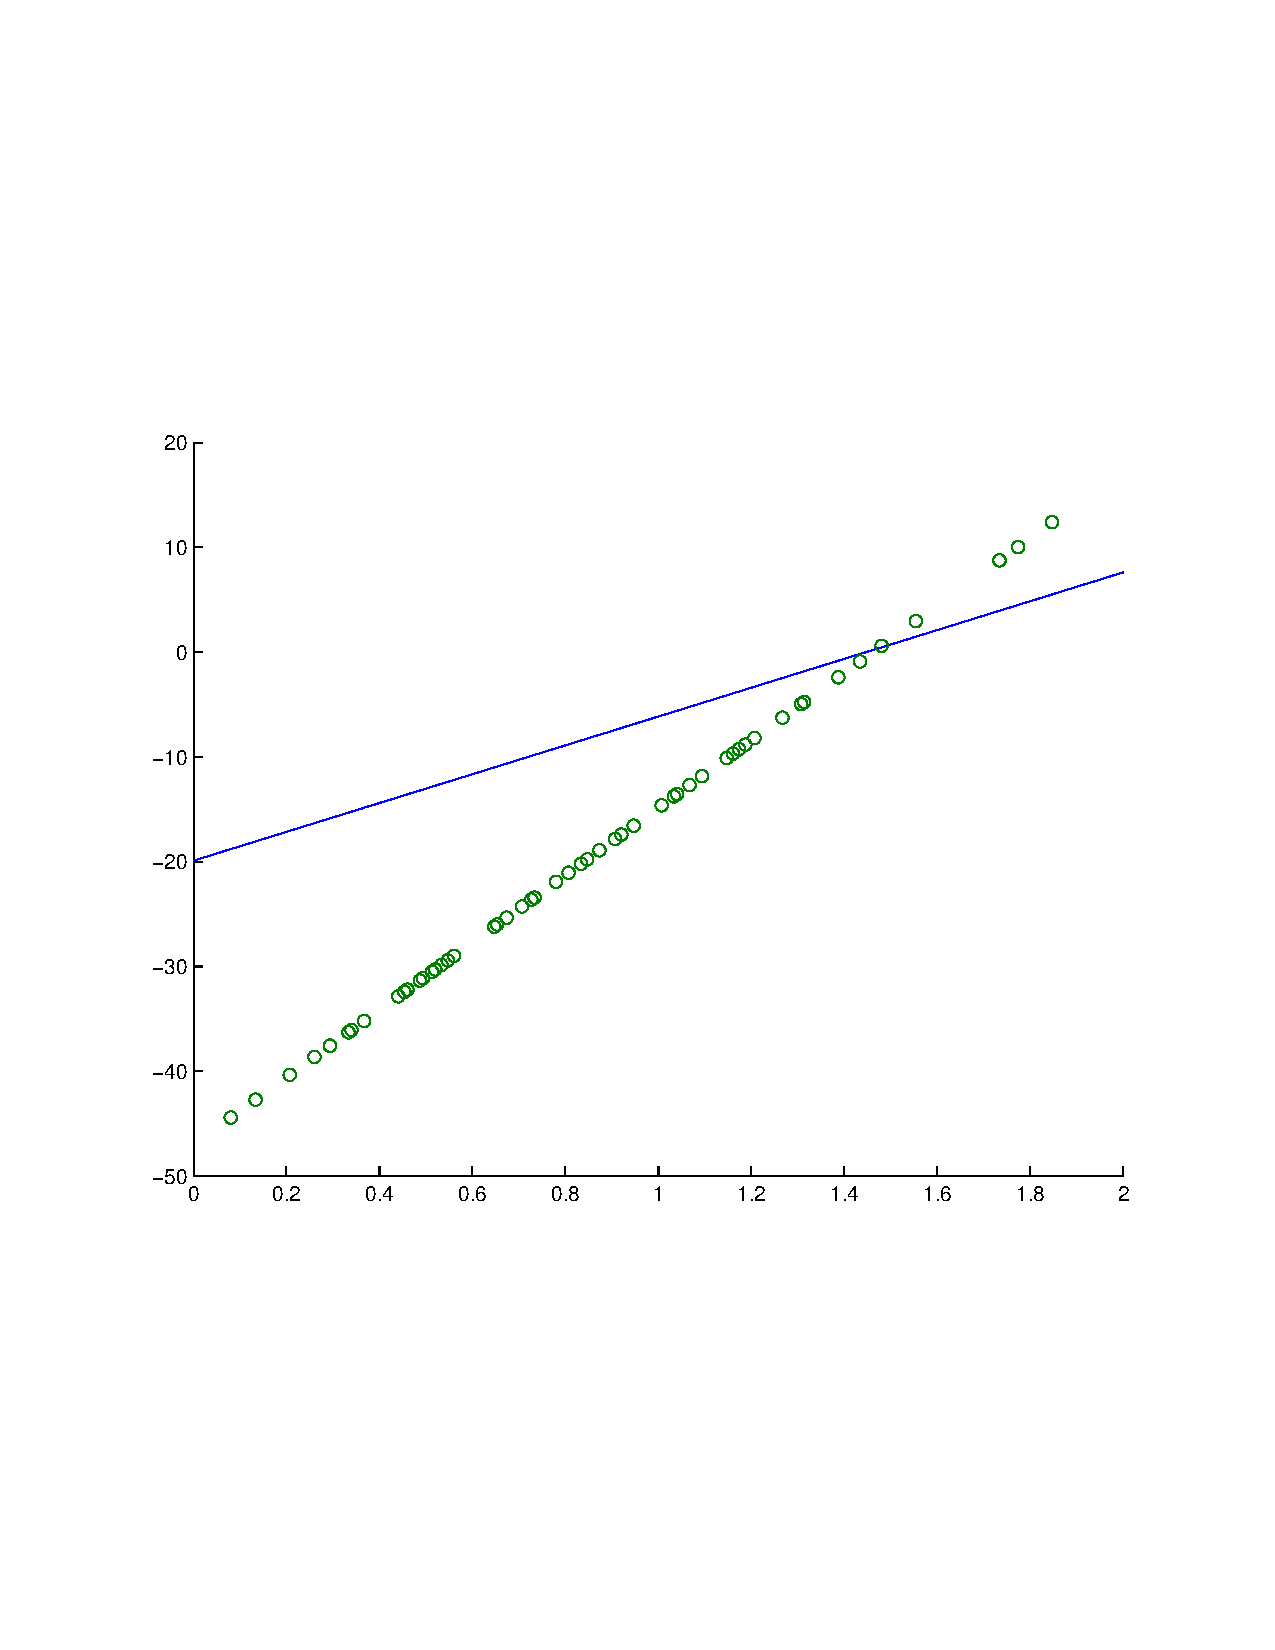
\includegraphics[width=.22\textwidth]{\figdir/prob1c_deg1} &
%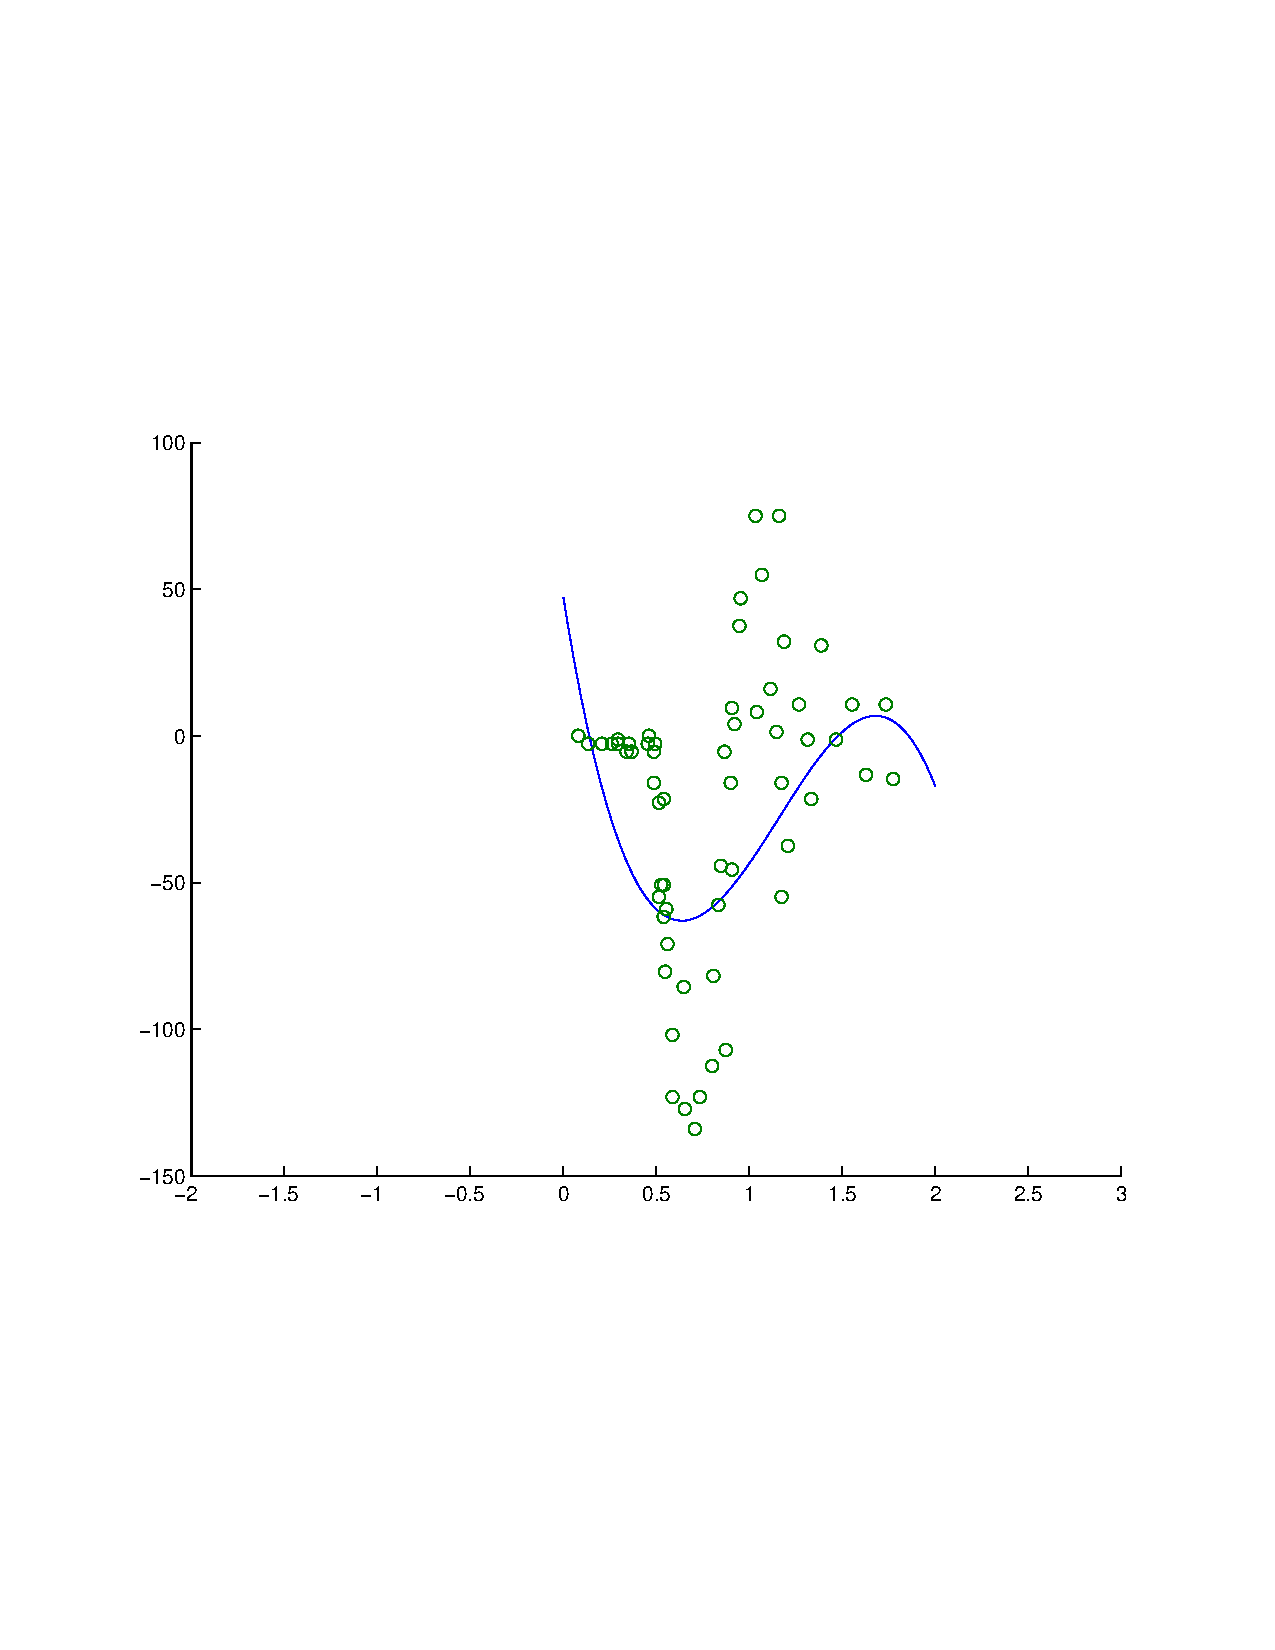
\includegraphics[width=.22\textwidth]{\figdir/prob1c_deg3} &
%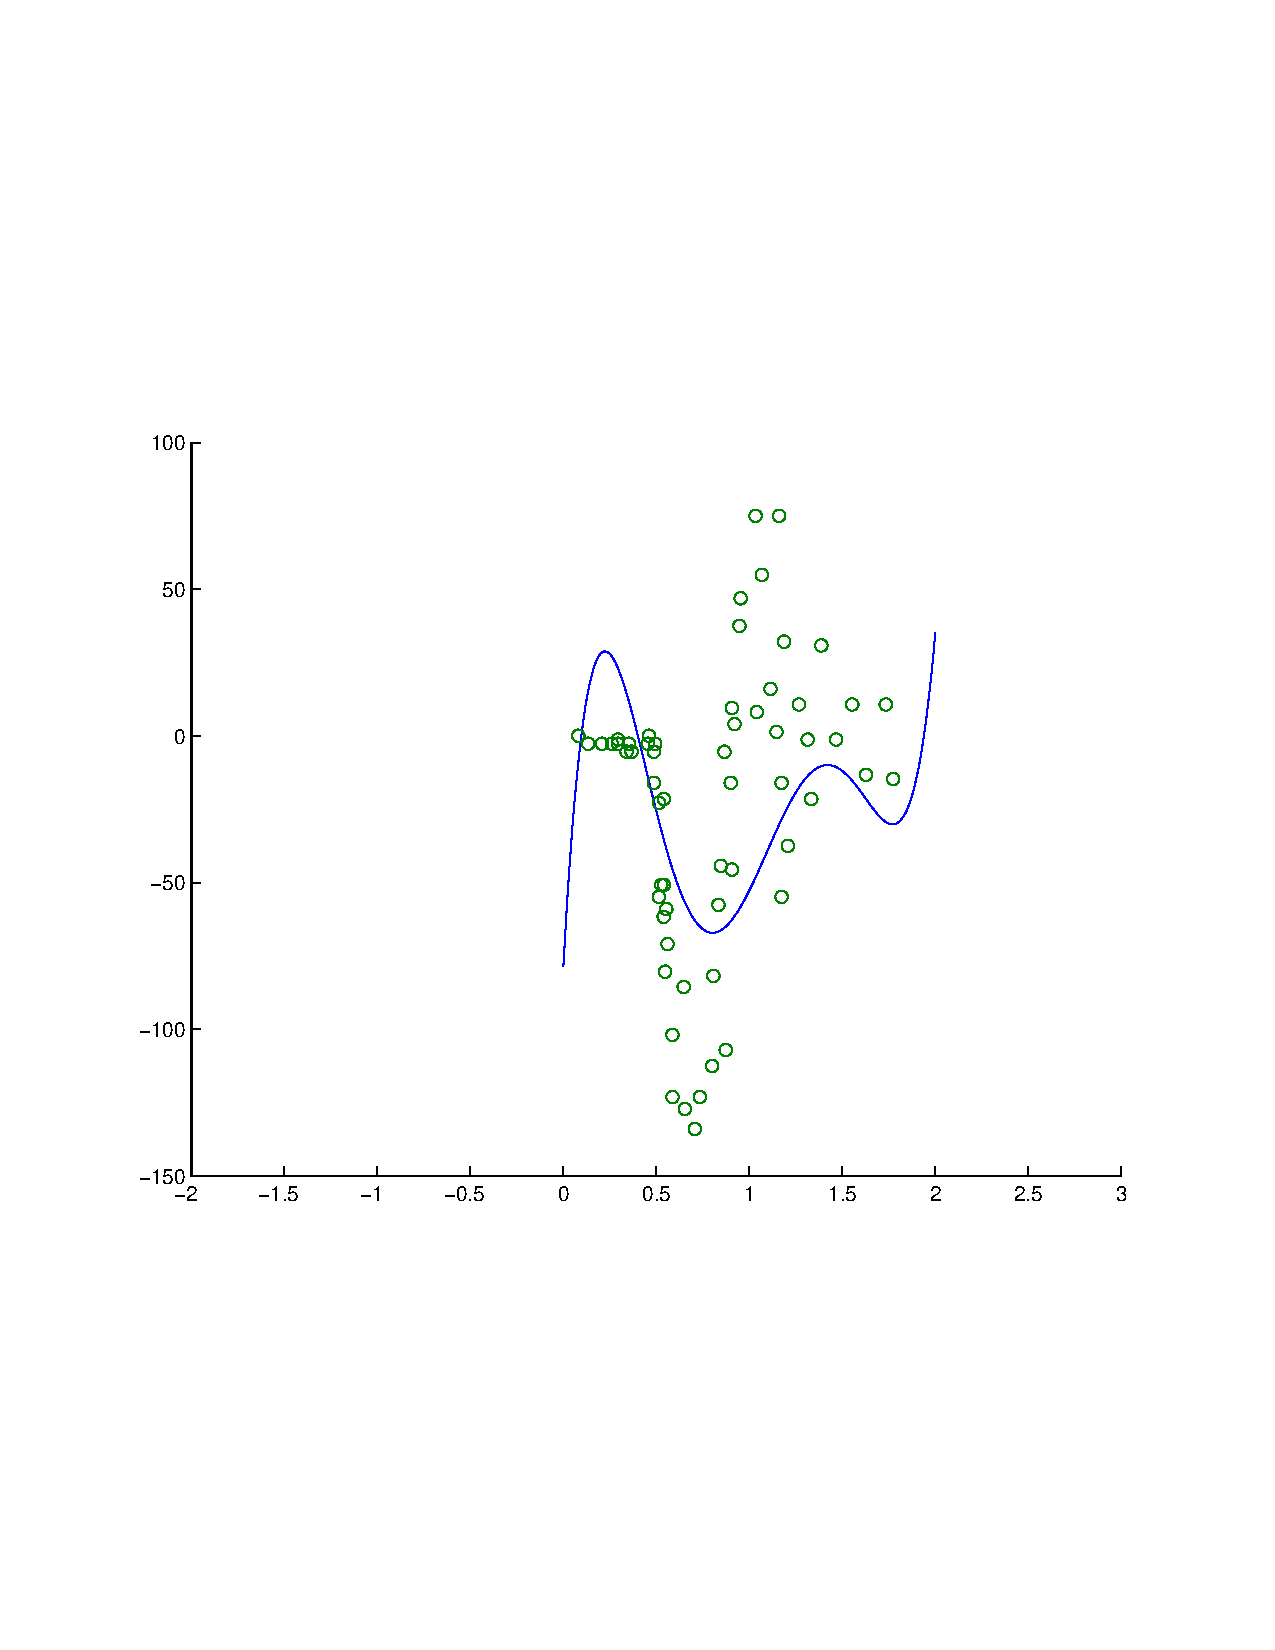
\includegraphics[width=.22\textwidth]{\figdir/prob1c_deg5} &
%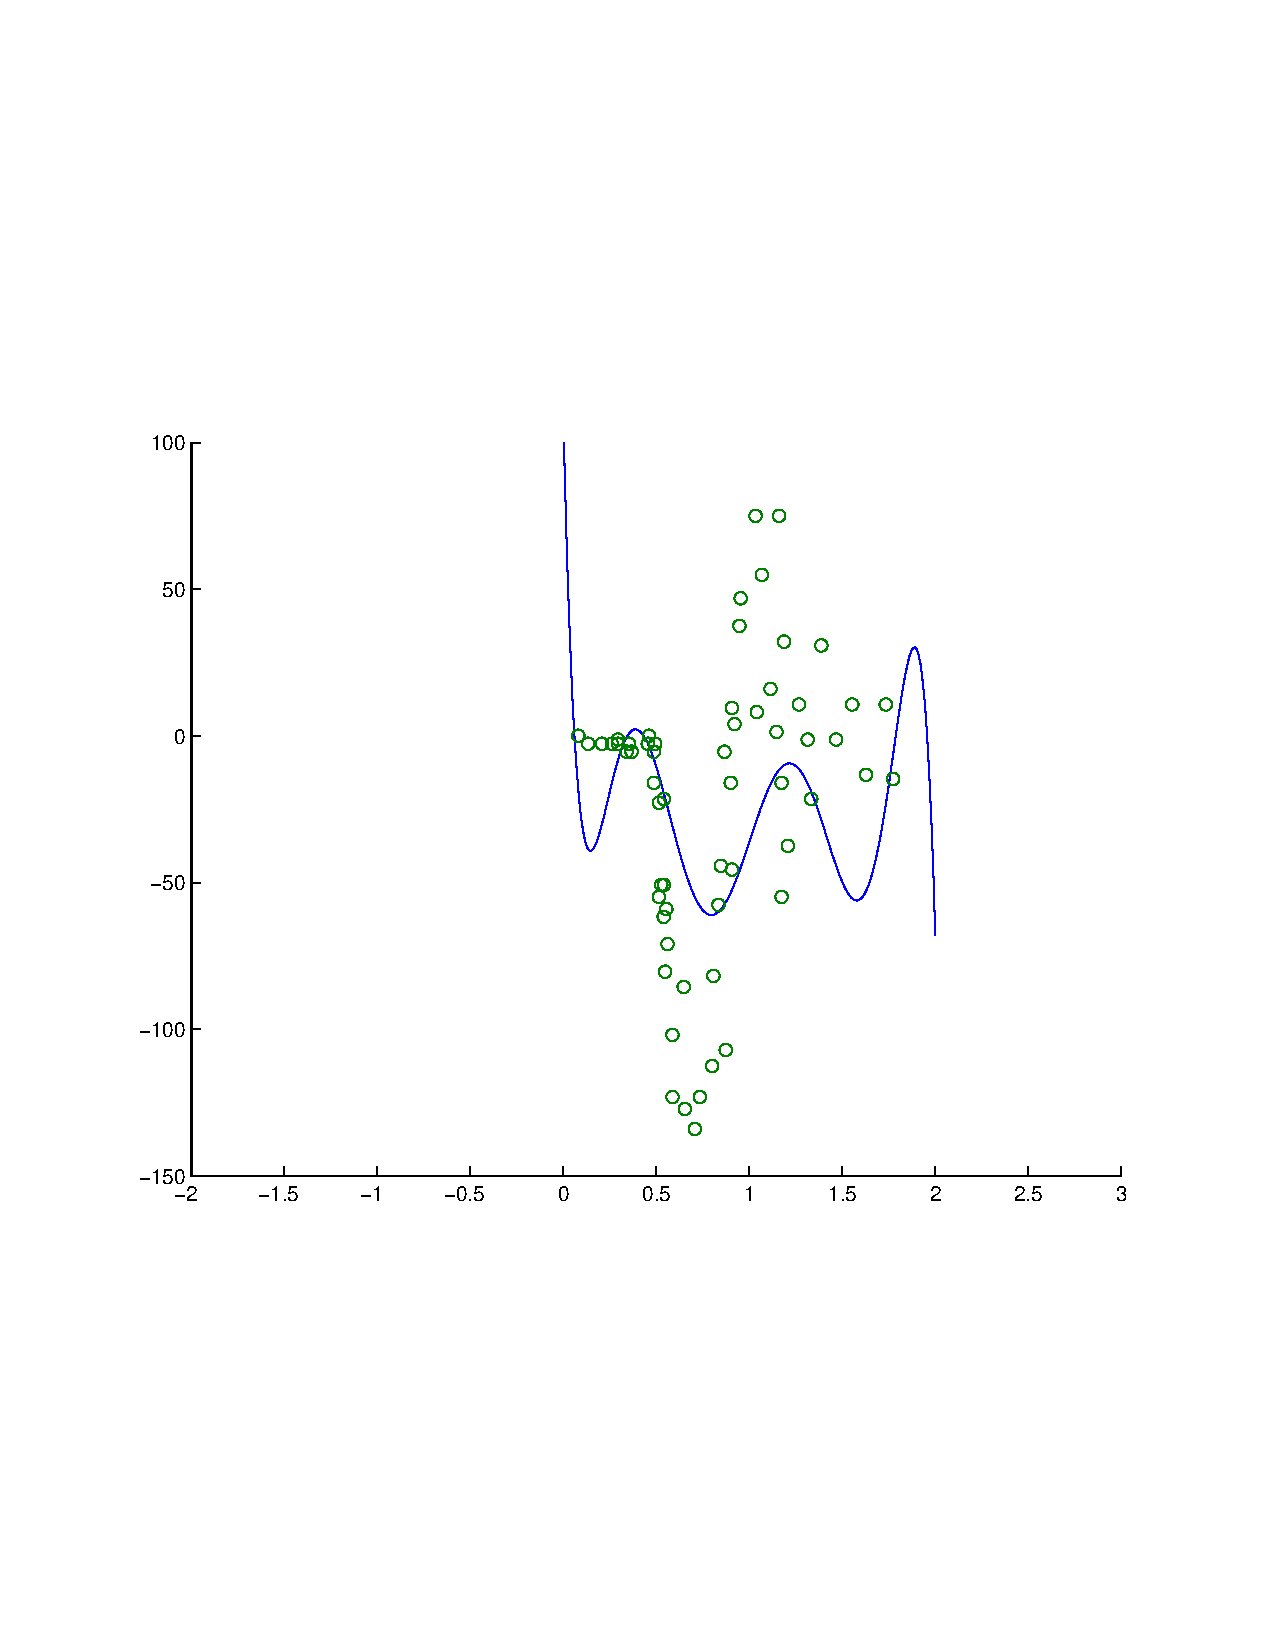
\includegraphics[width=.22\textwidth]{\figdir/prob1c_deg7} \\
%1 & 3 & 5 & 7 \\
%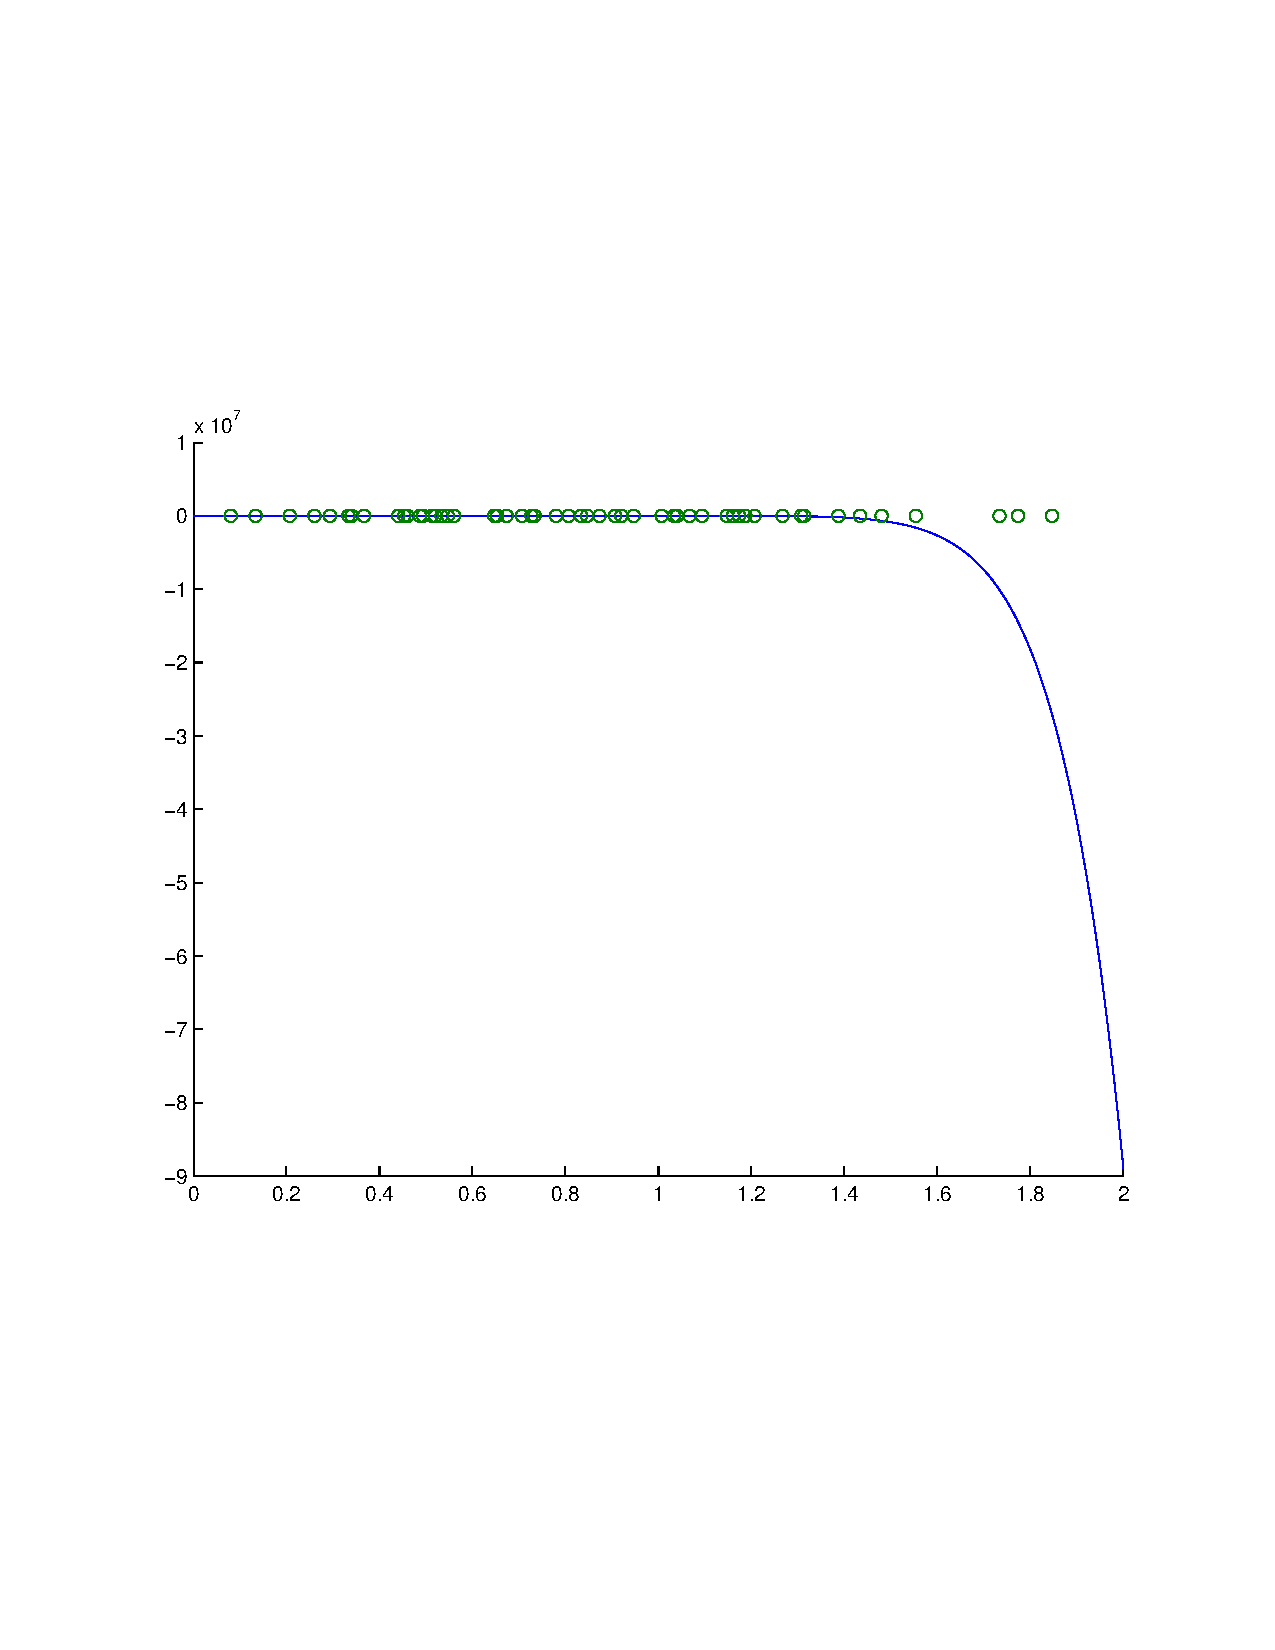
\includegraphics[width=.22\textwidth]{\figdir/prob1c_deg10} &
%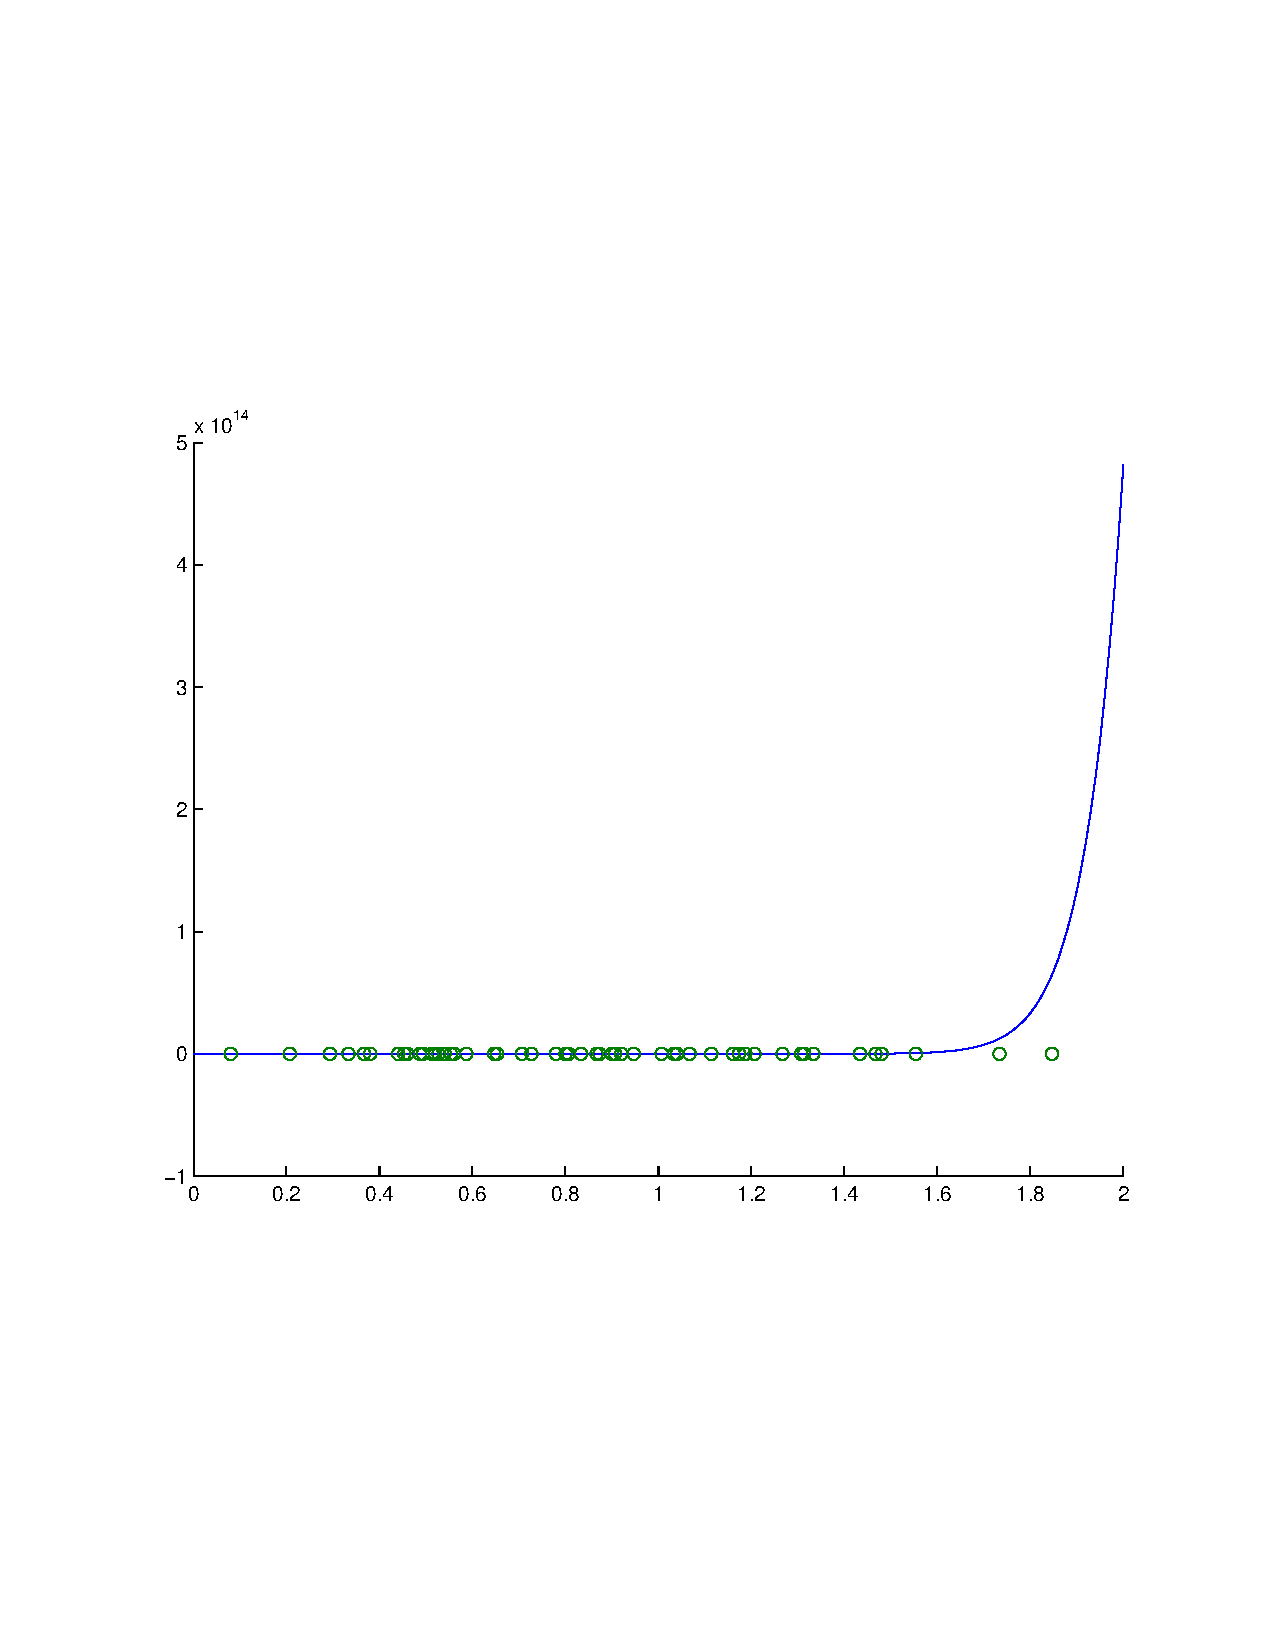
\includegraphics[width=.22\textwidth]{\figdir/prob1c_deg18} &
%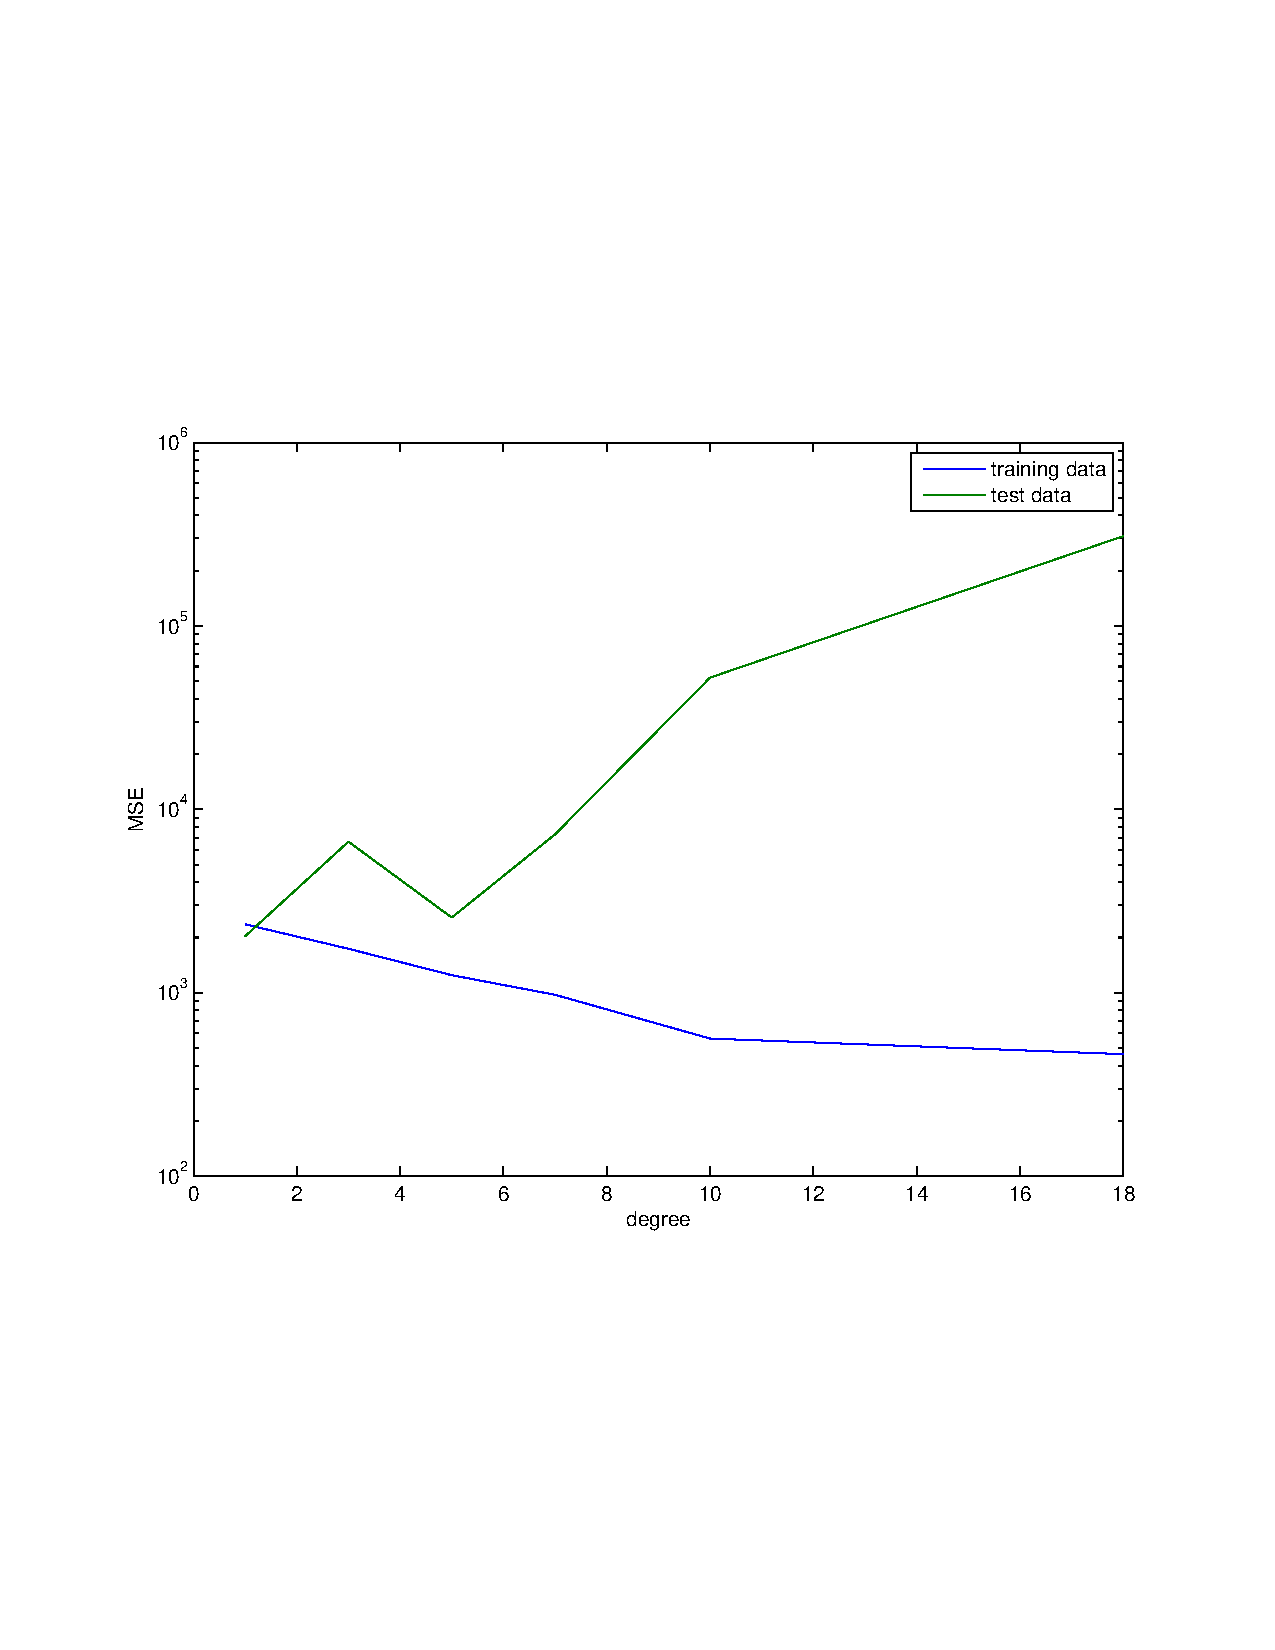
\includegraphics[width=.22\textwidth]{\figdir/prob1c_mse} \\
%10 & 18 & MSE
%\end{tabular}
%\end{figure}

\end{enumerate}

% % % % % % % % % % % % % % % % % % % % % % % % % % % % % % % % % % % % % % % % % % % % % % % % % % % % % % % % % % % % % % % %

\subsection*{Problem 2: Support Vector Machines}

\begin{enumerate}[(a)]
\item 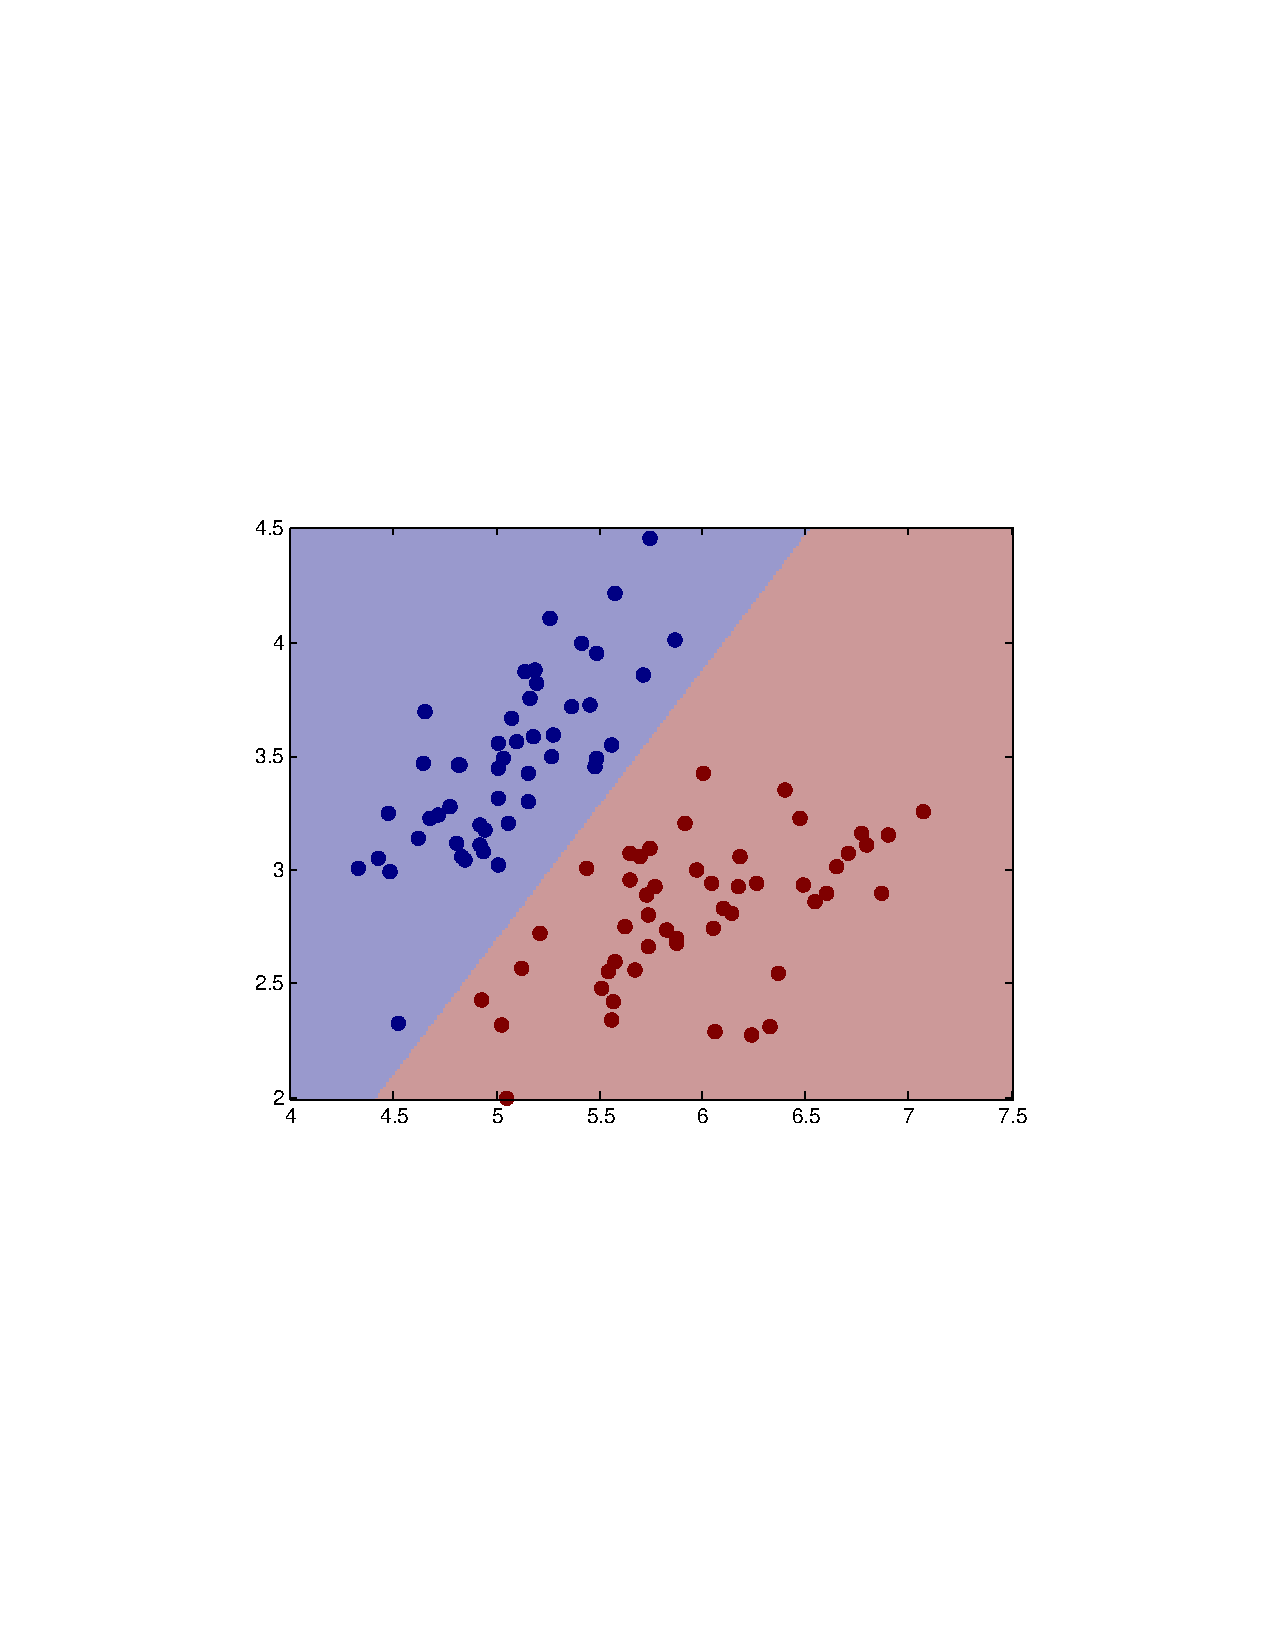
\includegraphics[width=.22\textwidth]{\figdir/prob2a}
\item TODO
%	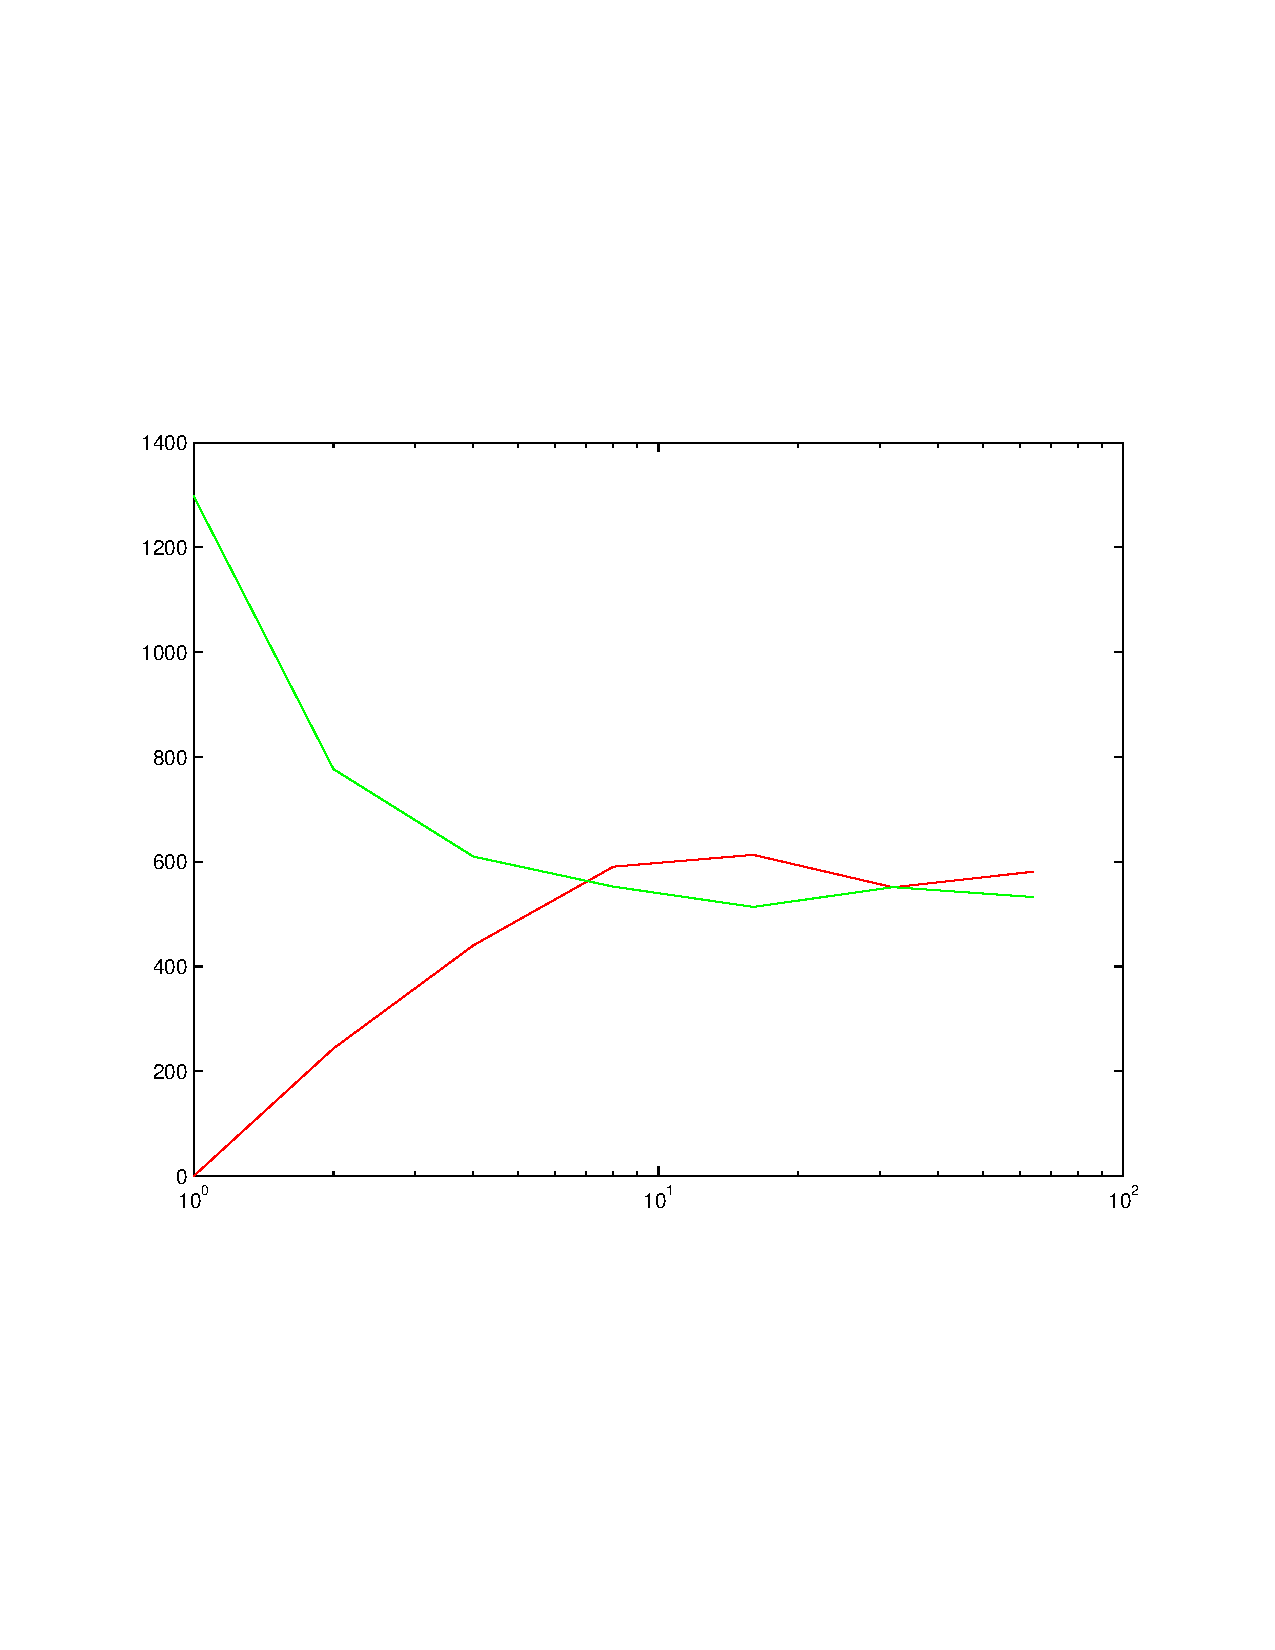
\includegraphics[width=.22\textwidth]{\figdir/prob2b}
\end{enumerate}

% % % % % % % % % % % % % % % % % % % % % % % % % % % % % % % % % % % % % % % % % % % % % % % % % % % % % % % % % % % % % % % %

\subsection*{Problem 3: Bagging with Decision Trees}

\begin{enumerate}[(a)]
\item Training error: 3.6219e-04 \\
Test error: 0.1565 \\
Settings: I uses nMin(0), infinite depth, minScore(.001), and all available features for splitting.

\item 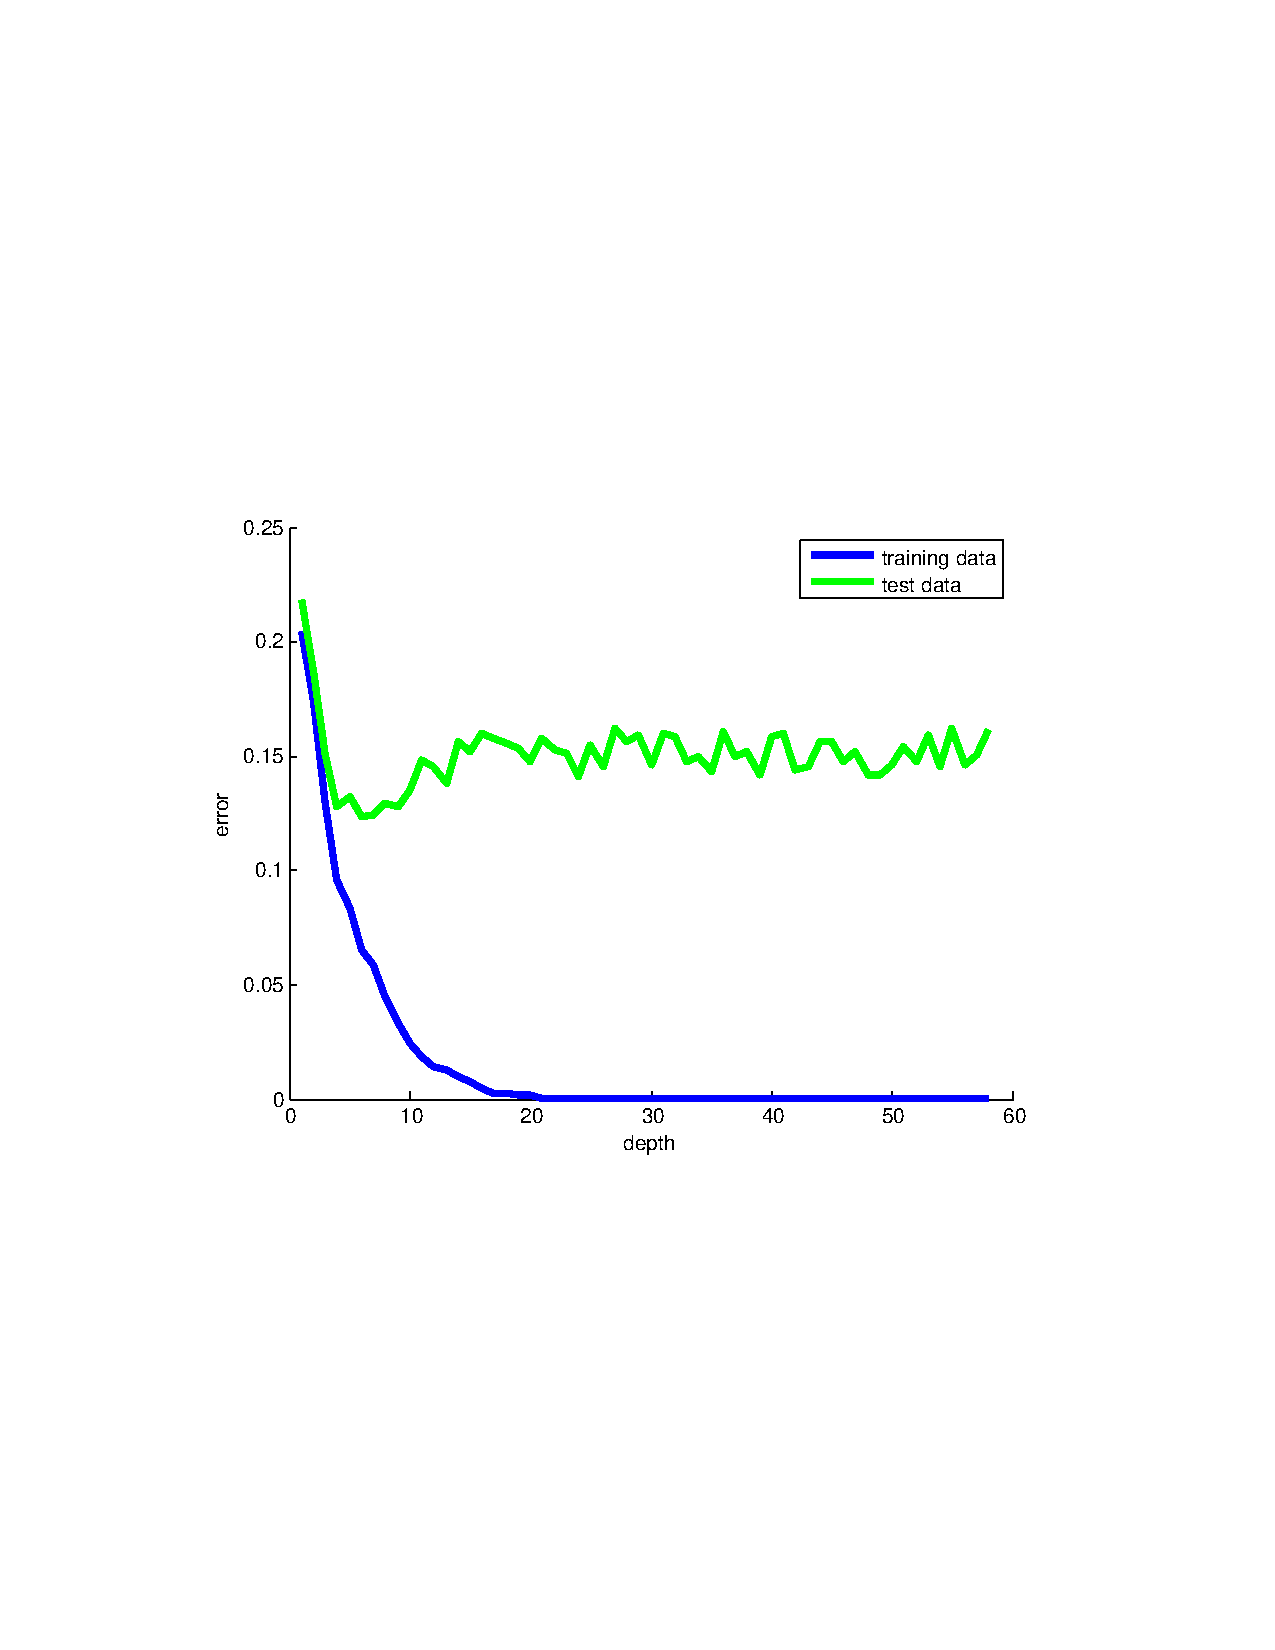
\includegraphics[width=.22\textwidth]{\figdir/prob3b}

\item We should believe that we are overfitting with these parameters because they introduce more complexity and, for example, learn training data completely with deep enough trees. \\
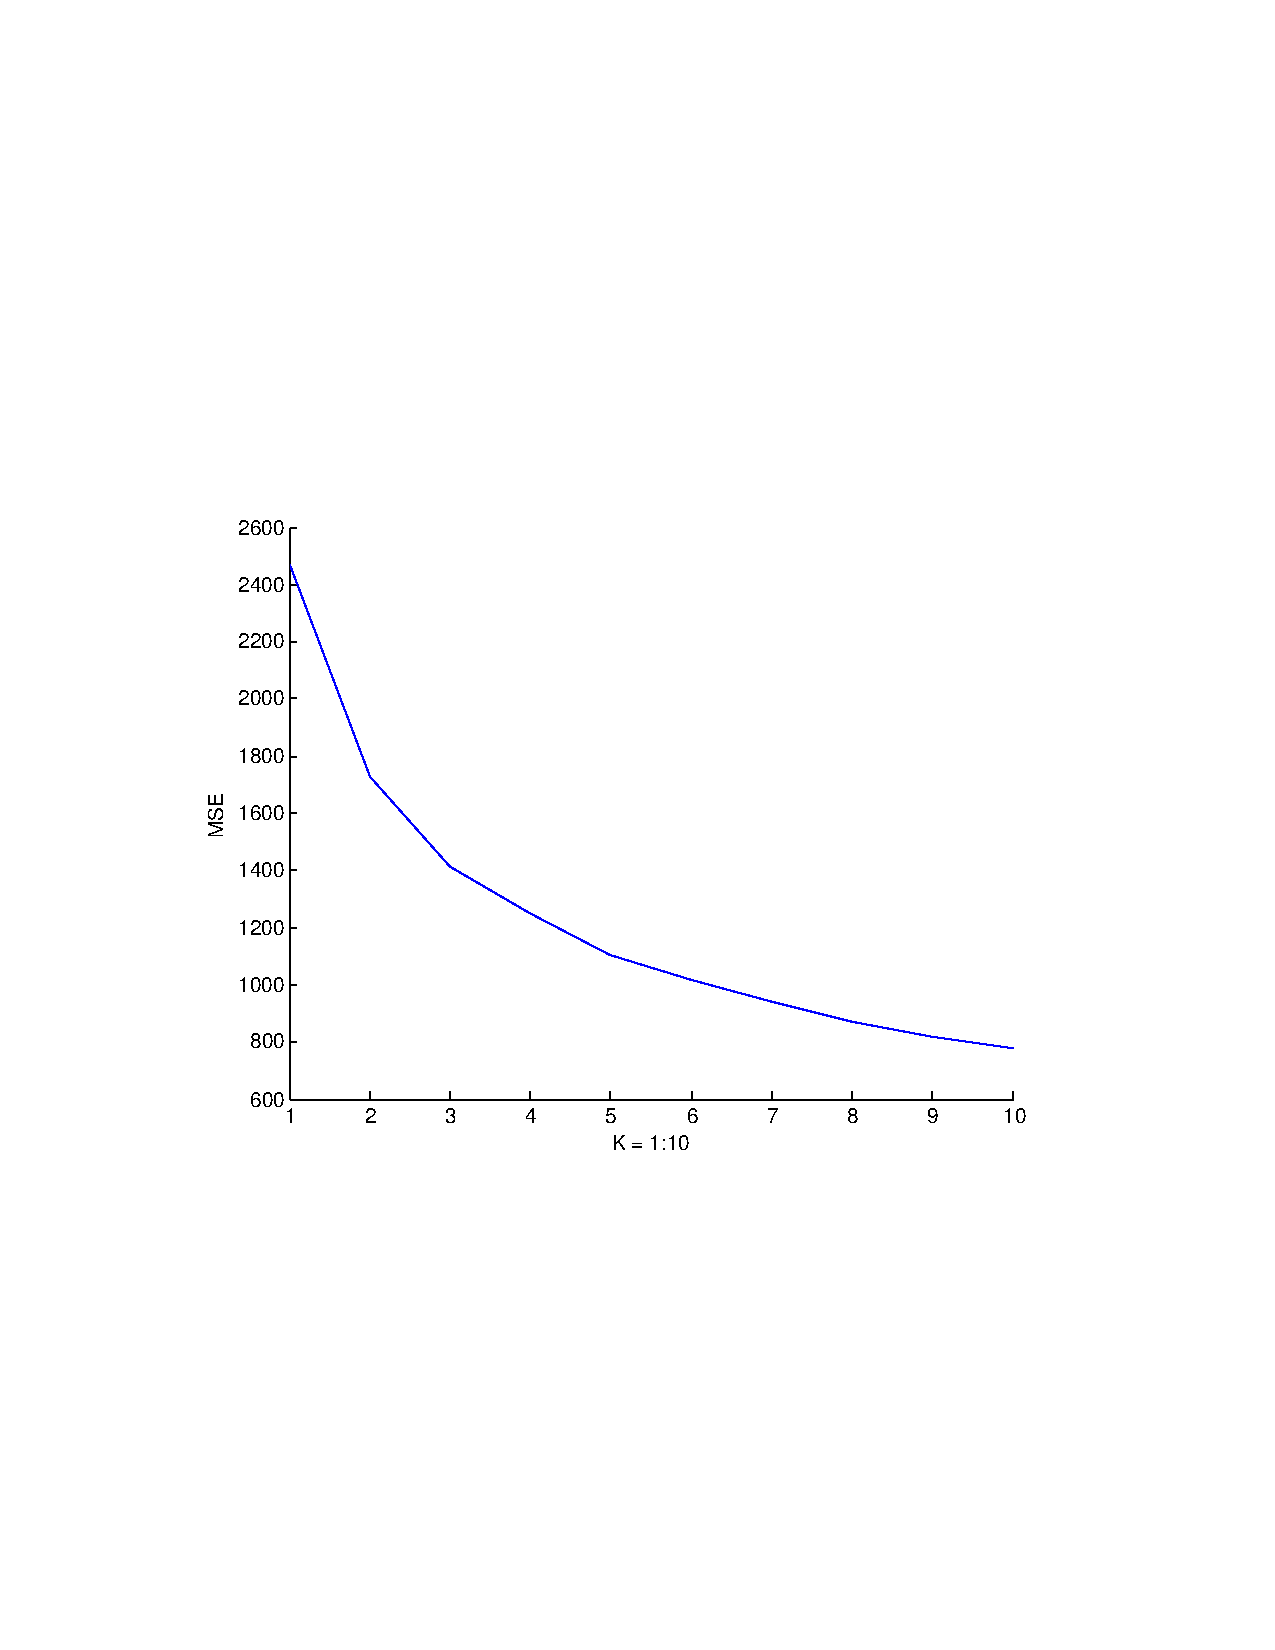
\includegraphics[width=.22\textwidth]{\figdir/prob3c}

\item In this figure we see that 
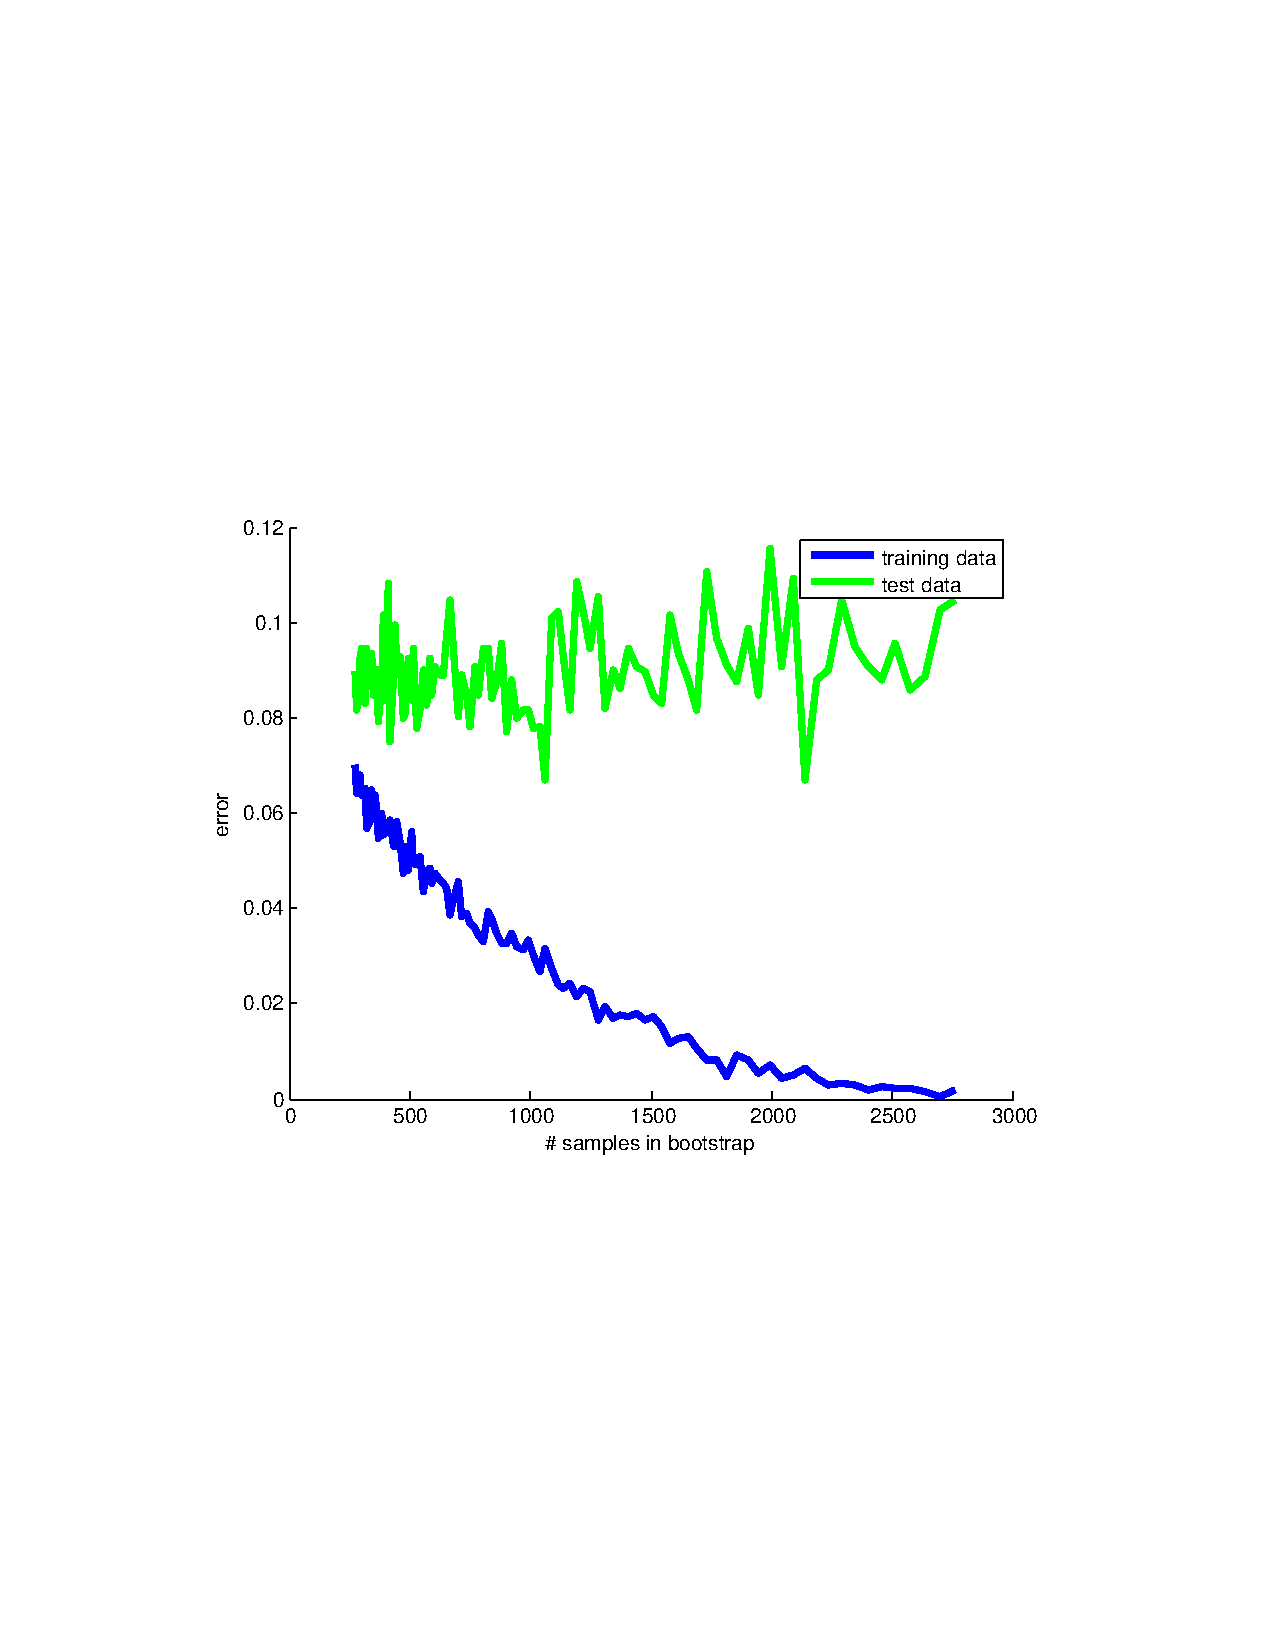
\includegraphics[width=.45\textwidth]{\figdir/prob3d}
\end{enumerate}

% % % % % % % % % % % % % % % % % % % % % % % % % % % % % % % % % % % % % % % % % % % % % % % % % % % % % % % % % % % % % % % %

\subsection*{Problem 4: Boosting}

\begin{enumerate}[(a)]
\item TBD
\end{enumerate}

\end{document}
